% Comments start with % (percent) character and last till the end of the line.
%
% The line below tells TeXworks editor to use pdflatex for compilation
% of this document; remove it if you want to use another engine 
%
%!TEX program = pdflatex
%
% LaTeX2e document starts with \documentclass[options]{<class-name>}
% <class-name> can be one of the standard LaTeX document classes: 
% article, report or book, or some other specialised class.
%
\documentclass[twocolumn]{article}
%
% Preamble of LaTeX document is everything before \begin{document}.
% Preamble is used to load extension packages and to set up global 
% parameters and configuration for the entire document.
%
% Extension packages providing additional functionality
\usepackage{amsmath}       % additional math environments
\usepackage{amsfonts}
\usepackage{graphicx}      % graphics import from external files 
\usepackage{epstopdf}      % automates .eps to .pdf conversion 
% epstopdf package may require --shell-escape option to pdflatex
\usepackage{booktabs}      % table typesetting additions
\usepackage{siunitx}       % number and units formatting
\usepackage{caption}       % customisation of captions
\usepackage{url}           % format url addresses
\usepackage{abstract}		% allows formatting of abstract
%\usepackage{tikz,pgfplots} % diagrams and data plots
%
% set up caption options
\captionsetup{margin=12pt,font=small,labelfont=bf}
%
%removes abstract title
\renewcommand{\abstractname}{}
%sets abstract margins
\setlength{\absleftindent}{30mm}
\setlength{\absrightindent}{30mm}
%
% global options for siunitx
%\sisetup{seperr,repeatunits=false,per=symbol}
%
% some handy commands for referencing;
% the optional argument overrides the default label, e.g.
% \figref[FIG.~]{fig:label}
\newcommand{\figref}[2][\figurename~]{#1\ref{#2}}
\newcommand{\tabref}[2][\tablename~]{#1\ref{#2}}
\newcommand{\secref}[2][Section~]{#1\ref{#2}}


% The document content starts with \begin{document} 
% and is finished with \end{document}
%
\begin{document}
\title{P01: Magnetic Monopoles} % fill in the title here
\author{John Morris}% fill in your name here
\date{January 2014} % date of the report
\twocolumn[	% makes title and abstract appear over entire page width
\maketitle % formats the title
\begin{onecolabstract}
\noindent
Dirac undertook a theoretical investigation magnetic monopoles, successfully determining their properties. The behaviour of electrically charged particles in the presence of monoples is susceptible to straightforward analysis. The paper then goes on to an analysis of the field itself. It will be seen that the axial nature of the magnetic field requires a different analysis to that applied in electrostatics.
\end{onecolabstract}
\vspace{5 mm}
]

\section{Introduction}
\label{sec:Introduction}
Dirac's symmetrised equations are defined in \cite{Paper01}. The equations are expressed in terms of potentials rather than fields. The Lorentz force and the obvious Coulomb-like equation both refer to fields. Further, the relationship $ \mathbf{B} =  \mathbf{\nabla} \times  \mathbf{A}$ may not be valid because $ \mathbf{B} = -  \mathbf{\nabla} \phi $ is expected to apply. Clearly, an eventual task will be to incorporate the existence of fields satisfying $ \mathbf{\nabla} \cdot  \mathbf{B} \neq 0$ into the theory.
\section{Charged particle motions}
\label{sec:Charged particles in a monopole field}
\subsection{Equation of motion}
An obvious start point is to define the magnetic field $\mathbf{B}$ by analogy with Coulomb's law:
\begin{equation}
\label{eq:E1}
\mathbf{B} = \frac {\mu_0 b}{4 \pi}\frac {\mathbf{r}}{r^3}
\end{equation}
It will then be assumed that the force on an electric charge $+e$ is given by:
\begin{equation}
\label{eq:E2}
\mathbf{F} = e ( \mathbf{\dot{r}} \times \mathbf{B} )
\end{equation}

\noindent
Combining these equations yields the following equation of motion:
\begin{equation}
\label{eq:E3}
\mathbf {\ddot{r}} = \frac {\mu_0 }{4 \pi } \frac {be}{m}\frac {\mathbf{\dot{r}} \times \mathbf{r}    }{r^3}
\end{equation}
An analysis of the solutions to this equation is given below.
\subsection{Solving the equation of motion}
$\mathbf{\ddot{r}}\cdot{\mathbf{\dot{r}}}$ and $\mathbf{\ddot{r}}\cdot{\mathbf{r}}$ are zero by the properties of the cross product. The first equation can be integrated to yield  $\mathbf{\dot{r}}\cdot{\mathbf{\dot{r}}}= v^2$, a constant. Thus the kinetic energy is a constant and, given that magnetic fields do no work on electrically charged particles, the total energy $E$ is also constant.

Integrating $\mathbf{\dot{r}}\cdot{\mathbf{\dot{r}}} $ with respect to $t$ gives $\mathbf{{r}}\cdot{\mathbf{\dot{r}}}= v^2 t$, where $\mathbf{{r}}\cdot{\mathbf{\dot{r}}}=0$ at $t=0$. A second integration gives $\mathbf{{r}}\cdot{\mathbf{{r}}}=r^2= v^2 t^2 + a^2$, where $a$ is the distance from the origin at $t=0$.

This analysis shows that there are no stable, localised orbits available to the particle except when $\mathbf r $ and $\mathbf{\dot{r}}$ are permanently perpendicular to each other. This most obviously occurs for vanishingly small orbits. This special case is explored below.
\subsection{Small orbit limit}
It is clear from the equation $\mathbf{{r}}\cdot{\mathbf{\dot{r}}}= v^2 t$ that the particle could remain localised for considerable periods of time if $v^2$ were small enough. In the limit $v^2$=0, $\mathbf{{r}}\cdot{\mathbf{\dot{r}}} $ would always be zero, suggesting a circular orbit. If this orbit were in the $xy$ plane it would be possible for the centripetal acceleration required to be supplied by the Lorentz force if the cross product produced a vector in this plane. This would occur in the limit of large $z$.
\noindent
Consider then a solution of the form:
\begin{equation}
\label{eq:E4}
\mathbf {{r}} = \rho \mathbf{\hat \rho }+z \mathbf{\hat k}
\end{equation}
\noindent
Differentiating with respect to $t$ and assuming $z$ is constant gives
$\mathbf {\dot{r}} = |\rho| \dot{\theta}  \mathbf{ \hat \theta }$. For a circular orbit $|\rho|$ and the angular frequency $\omega$ are constant. Combining with \eqref{eq:E3} leads to:

\begin{equation}
\label{eq:E5}
-\omega^2|\rho| \approx - \frac {\mu_0 be}{4 \pi m}\frac {\omega |\rho|z}{z^3}
\end{equation}

\noindent
Evidently $|\rho|$ drops out  to finally yield:
\begin{equation}
\label{eq:E6}
\omega \approx \frac {\mu_0 be}{4 \pi m z^2}
\end{equation}

\noindent
The solution corresponds to anti-clockwise rotation about $z$. Note that rotation in the opposite sense is not permitted because the cross product is an axial vector.

\subsection{Orbital angular momentum}
Differentiating $\mathbf{L} = m \mathbf{{r}} \times \mathbf{\dot r}$ with respect to time gives $\mathbf{\dot L} = m \mathbf r \times \mathbf {\ddot r}$. Combining this with \eqref{eq:E3} leads to:
\begin{equation}
\label{eq:E7}
\mathbf {\dot{L}}
= \frac {\mu_0 }{4 \pi } \frac {be}{m}
\frac {m \mathbf r \times ( \mathbf r \times \mathbf {\dot r})  } {r^3}
\end{equation}
This expands under the $BAC-CAB$ rule to :
\begin{equation}
\label{eq:E8}
\mathbf {\dot{L}}
= \frac {\mu_0 }{4 \pi }  {be}
\frac {\mathbf r  ( \mathbf r \cdot \mathbf {\dot r} )  - r^2 \mathbf {\dot r}   } {r^3}
= \frac {\mu_0 }{4 \pi }  {be} \frac {d} {dt} \frac {\mathbf r} {r}
\end{equation}
Integrating the expression for $\mathbf {\dot{L}}$ gives:
\begin{equation}
\label{eq:E9}
\mathbf {L} = \mathbf {L_0} + \frac {\mu_0 }{4 \pi } be  \mathbf {\hat r}
\end{equation}
$\mathbf {L}$ will besubject to quantization along  an arbitrary axis to give the result:
\begin{equation}
\label{eq:E10}
l_z = \frac {\mu_0 }{4 \pi \hbar }  {be} \in  \mathbb Z
\end{equation}
This differs from the Dirac quantization rule by a factor of $2$:
\begin{equation}
\label{eq:E11}
j = \frac {\mu_0 }{2 \pi  \hbar} {be} \in  \mathbb Z
\end{equation}
\noindent
The factor of $2$ presumably arises from the electron spin.
\subsection{Analytic solution}
The expression for $\mathbf {L}$ is the basis for a complete solution. Aligning $\mathbf {L_0} $ along the $z$ axis we obtain, via  \eqref{eq:E4} in cylindrical polar co-ordinates:
\begin{equation}
\label{eq:E12}
\mathbf {\dot{r}} =\dot{ \rho} \mathbf{\hat \rho }+\rho \dot{\theta}  \mathbf{ \hat \theta } + \dot{z} \mathbf{\hat k} 
\end{equation}
Forming the cross product $\mathbf{L} = m \mathbf{{r}} \times \mathbf{\dot r}$ we find:
\begin{equation}
\label{eq:E13}
L_\rho = -mz \rho \dot {\theta} = \frac {\mu_0 }{4 \pi } be \frac {\rho}{\sqrt{\rho^2+z^2}}
\end{equation}
\begin{equation}
\label{eq:E14}
L_\theta  = m ( z \dot\rho-\rho\dot z) = 0
\end{equation}
\begin{equation}
\label{eq:E15}
L_z  = m \rho^2 \dot\theta = L_0 + \frac {\mu_0 }{4 \pi } be \frac {z}{\sqrt{\rho^2+z^2}}
\end{equation}
Equation \eqref{eq:E14} can be integrated to give $\rho = z \tan\alpha$, showing that the particle is confined to the surface of a cone whose apex isat the origin, of semi-angle $\alpha$ whose axis is parallel to $\mathbf {L_0}$. Multiplying \eqref{eq:E13} by $\rho$, \eqref{eq:E15} by $z$ and adding gives:
\begin{equation}
\label{eq:E16}
L_\rho \rho +L_z z = 0= L_0 z  + \frac {\mu_0 }{4 \pi } be \sqrt{\rho^2+z^2}
\end{equation}
Evidently $ \sqrt{\rho^2+z^2} = z \sec\alpha $ so that:
\begin{equation}
\label{eq:E17}
\cos \alpha = - \frac {\mu_0 }{4 \pi } be \frac{1}{L_0}
\end{equation}
From \eqref{eq:E12}, $\mathbf {\dot{r}} \cdot \mathbf {\dot{r}} = v^2 = \dot\rho^2 +\rho^2\dot\theta^2 +\dot z^2 $ and using $ \dot\rho = \dot z \tan\alpha$ we obtain $v^2 = \dot z^2 \sec^2 \alpha + z^2\dot \theta^2 \tan^2 \alpha$. After some algebra we find:
\begin{equation}
\label{eq:E18}
\dot z = v \cos\alpha ( 1 - ({L_0 \sin\alpha \cos\alpha}/{mvz})^2)^\frac{1}{2}
\end{equation}
Writing $z_0 = {L_0 \sin\alpha \cos\alpha}/{mv}$ this reduces to:
\begin{equation}
\label{eq:E19}
\dot z = v \cos\alpha ( 1 - ({z_0}/{z})^2)^\frac{1}{2}
\end{equation}
Thus $z_0$ and the corresponding $\rho_0=z_0 \, tan\alpha$ represent the locus of the closest points to the origin the particle can reach. Further algebra shows that $z^2 = z_0^2 + v^2 t^2 \cos^2\alpha$ and $\rho^2 = \rho_0^2 + v^2 t^2 \sin^2\alpha$. Finally, \eqref{eq:E13} reduces to:
\begin{equation}
\label{eq:E20}
\dot\theta = - \frac{L_0}{m}\cos^2\alpha\frac{1}{z^2}
\end{equation}
Substituting for $z^2$ we find:
\begin{equation}
\label{eq:E21}
\theta(t) = \int_0^t - \frac{L_0}{m} \cos^2\alpha \frac{1}{z_0^2 +v^2t^2\cos^2\alpha} \,\mathrm{d}t
\end{equation}
This integral can be evaluated via the substitution $\tan u = vt\cos\alpha/z_0$ to give:
\begin{equation}
\label{eq:E22}
\theta(u) = \int_0^u - \frac{L_0}{m} \cos^2\alpha  \frac{1}{z_0^2 \sec^2u} \frac{z_0}{v\cos\alpha} \sec^2u\,\mathrm{d}u
\end{equation}
and finally:
\begin{equation}
\label{eq:E23}
\theta(u) = - \frac{L_0u}{mvz_0} \cos\alpha
\end{equation}
A complete solution in parametric form has therefore been found.
\subsection{Particle paths in space}
The general features of the path may be inferred from the equations:
\begin{itemize}
  \item The path lies on the surface of a cone whose apex is at the origin and whose axis is aligned with $\mathbf L_0$.
  \item There is a minimum distance that the particle may get to the origin.
  \item There are no bound states, so all particle paths start and end at $\infty$.
\end{itemize}
\noindent
The chart below illustrates a typical particle path:
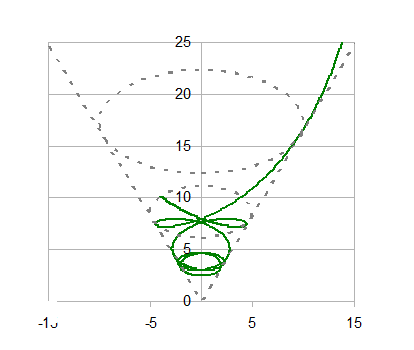
\includegraphics[width=80mm]{mm1.jpg}
The projection of this path onto the $xy$, $yz$ and $zx$ planes shows the orbit around the $z$ axis more clearly:
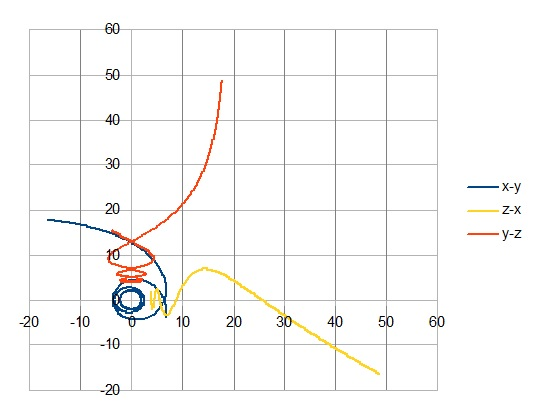
\includegraphics[width=80mm]{mm2.jpg}
A close-up iof the central region is shown below:
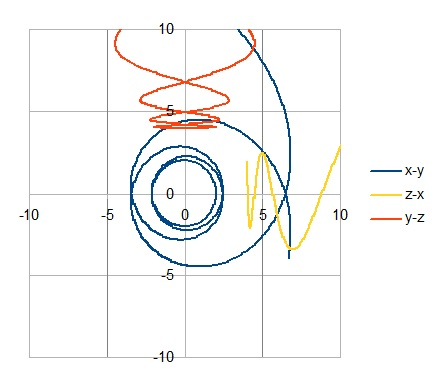
\includegraphics[width=80mm]{mm3.jpg}
The requirement that the particle path lie on the surface of a cone is clearly shown in the $yz$ projection in isolation:
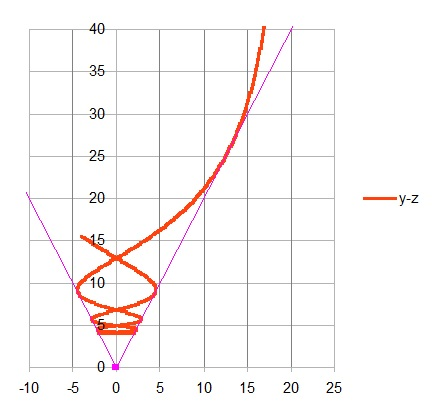
\includegraphics[width=80mm]{mm4.jpg}
This projection in particular shows the tendency to execute several near planar orbits at closest approach before receding to infinity.
\section{Monopole field equations}
\label{sec:Field equations}
\subsection{Characteristics of the field}
The electric field from a point electric charge is given by  $\mathbf E = -\nabla \phi_e$. Similarly, it is to be expected that the magneticfield from a point magnetic field would be given by  $\mathbf B = -\nabla \phi_b$.

\noindent
$\nabla \times \mathbf E = 0$ holds for static electric fields and electric charges. However, it is not true that $\nabla \times \mathbf B = 0$ since $\mathbf B$ is an axial vector. It follows that the potential associated with a point magnetic charge must be capable of generating such a vector. The scalar nature of a point electric charge does not permit this. It follows that a point magnetic charge cannot be modelled as a scalar.

\noindent
$\mathbf B$ is associated with a magnetic potential $\mathbf A$ such that $\nabla \times \mathbf A = \mathbf B$ in standard magnetostatics. Just as $\phi$ is associated with a point electric charge to give rise to $\mathbf E$, so $\mathbf A$ will be associated with a point magnetic charge to give rise to  $ \mathbf B$. The task then is to find an $\mathbf A$ satisfying $\nabla \times \mathbf A = \mathbf B$ which results in a $\mathbf B$ which drops off as $1/r^2$, is parallel to the radius vector from the magnetic charge and which generates the desired axial nature of $\mathbf B$.

\subsection{Semi-infinite solenoid}
It is well known that a solenoid produces a magnetic field externally identical to that produced by a magnetic dipole:

\noindent
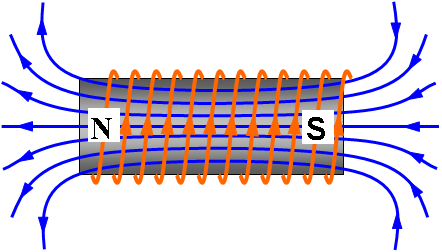
\includegraphics[width=80mm]{solenoid.png}

\noindent
In the extreme case that the solenoid is of semi-infinite length, deach pole take on the characteristics of isolated magnetic monoples. Moreover, because the field is generated by a current the requirement that there be a vector potential $\mathbf A$ satisfying $\nabla \times \mathbf A = \mathbf B$ will be met.

\newpage
\begin{thebibliography}{9}
\bibitem{Paper01} \emph{ME07 Euler Strut} Provided Material
\end{thebibliography}
\end{document}
